\documentclass[12pt]{article}

\usepackage{amsmath}
\usepackage{amssymb}
\usepackage{graphicx}
\usepackage{listings}
\usepackage{xcolor}
\usepackage{geometry}
\usepackage{hyperref}
\usepackage{enumitem}
\usepackage{caption}
\usepackage{booktabs}
\usepackage{array}
\usepackage{tikz}
\usetikzlibrary{arrows.meta, positioning, calc}
\usepackage{textcomp}

\graphicspath{{./screenshots/}}
\geometry{margin=1in}
\setlength{\parindent}{0pt}
\setlength{\parskip}{6pt}
\setcounter{secnumdepth}{0}
\tolerance=1000
\emergencystretch=\maxdimen

\lstset{
    basicstyle=\ttfamily\small,
    keywordstyle=\color{blue},
    commentstyle=\color{gray},
    stringstyle=\color{orange},
    numbers=left,
    numberstyle=\tiny,
    breaklines=true,
    columns=fullflexible,
    frame=single,
    backgroundcolor=\color{gray!10}
}

\begin{document}

\begin{center}
    {\LARGE \textbf{RBE 500 -- Homework 6}} \\[6pt]
    {\large Tracy Yang} \\[4pt]
    {\large \today}
\end{center}

%=============================================================
\section{Problem: Robot Control}

Consider the closed-loop control system below, where $x_r$ is the
reference position, $e$ is the error, $u$ is the control effort, and
$x$ is the resulting system output.

\begin{center}
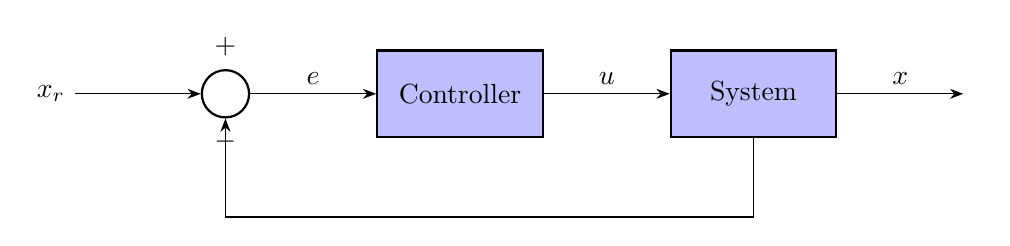
\begin{tikzpicture}[
    >=Stealth,
    block/.style = {draw, thick, minimum width=2.1cm, minimum height=1.1cm, align=center, fill=blue!25},
    sum/.style   = {draw, thick, circle, minimum size=0.6cm, inner sep=0pt},
    node distance = 1.6cm and 1.6cm
]
    \node (input) {$x_r$};
    \node[sum, right=of input] (sum) {};
    \node[block, right=of sum] (controller) {Controller};
    \node[block, right=of controller] (system) {System};
    \node[right=of system] (output) {};

    \draw[->] (input) -- (sum);
    \draw[->] (sum) -- node[above]{$e$} (controller);
    \draw[->] (controller) -- node[above]{$u$} (system);
    \draw[->] (system) -- node[above]{$x$} (output);

    \draw (sum.north) node[above=0.05cm]{$+$};
    \draw (sum.south) node[below=0.05cm]{$-$};

    % feedback line
    \coordinate (fbdown) at ($(system.south) + (0,-1.0)$);
    \draw[->] (system.south) |- (fbdown) -| (sum.south);
\end{tikzpicture}
\end{center}

The system dynamics are given by
\[
m\ddot{x} + b\dot{x} = u,
\]
and the controller is a PD (proportional--derivative) law
\[
k_p e + k_d \dot{e} = u.
\]

%-------------------------------------------------------------
\subsection{Part a) Laplace Domain}

Taking the Laplace transform of both differential equations, with
zero initial conditions ($x(0)=0$, $\dot x(0)=0$, $e(0)=0$), and
using $\mathcal{L}\{\dot f(t)\} = sF(s)$, $\mathcal{L}\{\ddot
f(t)\} = s^2F(s)$:

\textbf{System model:}
\[
m\ddot{x}+b\dot{x}=u
\quad\xrightarrow{\;\mathcal{L}\;}\quad
m\,s^2 X(s) + b\,s\,X(s) = U(s)
\]
\[
\boxed{(ms^2+bs)\,X(s) = U(s)}
\]

\textbf{Controller:}
\[
k_p e + k_d \dot e = u
\quad\xrightarrow{\;\mathcal{L}\;}\quad
k_p E(s) + k_d\, s\, E(s) = U(s)
\]
\[
\boxed{(k_p+k_d s)\,E(s) = U(s)}
\]

%-------------------------------------------------------------
\subsection{Part b) Transfer Functions}

\textbf{Controller transfer function} $\dfrac{U(s)}{E(s)}$:

From $(k_p+k_d s)E(s) = U(s)$,
\[
\boxed{\dfrac{U(s)}{E(s)} = k_p + k_d s}
\]

\textbf{System transfer function} $\dfrac{X(s)}{U(s)}$:

From $(ms^2+bs)X(s) = U(s)$,
\[
\boxed{\dfrac{X(s)}{U(s)} = \dfrac{1}{ms^2+bs} = \dfrac{1}{s(ms+b)}}
\]

\textbf{Forward (open-loop) transfer function} $\dfrac{X(s)}{E(s)}$:

Since $X(s)/E(s) = \big[X(s)/U(s)\big]\cdot\big[U(s)/E(s)\big]$,
\[
\boxed{\dfrac{X(s)}{E(s)} = \dfrac{k_p+k_d s}{ms^2+bs} = \dfrac{k_d s + k_p}{s(ms+b)}}
\]

%-------------------------------------------------------------
\subsection{Part c) Closed-Loop Transfer Function}

From the block diagram, the error is $e = x_r - x$, i.e.
\[
E(s) = X_r(s) - X(s).
\]

Substituting into the forward transfer function found in part (b):
\[
X(s) = \dfrac{k_p+k_d s}{ms^2+bs}\,\big[X_r(s) - X(s)\big]
\]

Distribute and collect all $X(s)$ terms on the left-hand side:
\[
(ms^2+bs)\,X(s) = (k_p+k_d s)\,X_r(s) - (k_p+k_d s)\,X(s)
\]
\[
\big[ms^2+bs+k_p+k_d s\big]\,X(s) = (k_p+k_d s)\,X_r(s)
\]
\[
\big[ms^2+(b+k_d)s+k_p\big]\,X(s) = (k_d s+k_p)\,X_r(s)
\]

Therefore the closed-loop transfer function is
\[
\boxed{\dfrac{X(s)}{X_r(s)} = \dfrac{k_d s + k_p}{m s^2 + (b+k_d)s + k_p}}
\]

\end{document}